% Images for Introductory Chemistry (c) by Dale J. Brugh

% Images for Introductory Chemistry is licensed under a
% Creative Commons Attribution-ShareAlike 4.0 International License.

% You should have received a copy of the license along with this 
% work. If not, see http://creativecommons.org/licenses/by-sa/4.0/.

\documentclass[tikz,varwidth=true,border=2pt]{standalone}
\usepackage[T1]{fontenc}
\renewcommand{\rmdefault}{ptm}	% Sets roman font to Times
\usepackage[scaled=0.92]{helvet}
\usepackage[subscriptcorrection,slantedGreek,nofontinfo,mtpcal]{mtpro2}
\usetikzlibrary{arrows}
\begin{document}
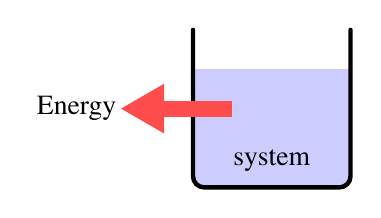
\begin{tikzpicture}
\draw[fill=blue!20!white, rounded corners, draw=none] (0,-0.5) rectangle (2,-2);
\draw[fill=blue!20!white, draw=none] (0,-0.5) rectangle (2,-1);
\draw [rounded corners,ultra thick,cap=round] (0,0) -- (0,-2) -- (2,-2) -- (2,0);
\node [below] at (1,-1.4) {system};
\path[draw=red!70,solid,line width=2mm,fill=red!80,
preaction={-triangle 60,draw=red!70,shorten >= -6mm}
] (0.5, -1) -- (-0.5, -1);
\node [left] at (-0.85,-1) {Energy};
\end{tikzpicture}
\end{document}